\input ../SlidePreamble
\input ../preamble


\begin{document}

{\Huge

  \centerline{\bf TTIC 31230, Fundamentals of Deep Learning}
  \bigskip
  \centerline{David McAllester, Winter 2020}
  \vfill
  \centerline{\bf Generative Adversarial Networks (GANs)}
\vfill
\vfill


\slide{The Fundamental Equation for Continuous $y$}

If $y$ is continuous then the fundamental equation for estimating the distribution on $y$ (cross entropy) involves continuous probability densities.

\vfill
$$\Phi^* = \argmin_\Phi \;E_{y \sim \popd}\;-\ln p_\Phi(y)$$

\vfill
This occurs in unsupervised pretraining for sounds and images.

\vfill
But differential entropy and differential cross-entropy are conceptually problematic.

\slide{Generative Adversarial Networks (GANs)}

GANs avoid the differential cross-entropy loss function.

\vfill
The model distribution $p_\Phi(y)$ is represented by a generator and the objective function involves a
discriminator in place of cross-entropy.

\anaslide{Representing a Distribution with a Generator}

\bigskip
\centerline{$z$\hspace{5in}$y_\Phi(z)$}
\centerline{\includegraphics[width=6in]{\images/generator2}}

\bigskip
The random input $z$ defines a probability density on images $y_\Phi(z)$.  We will write this as $p_\Phi(y)$ for the image $y$.

\anaslide{Representing a Distribution with a Generator}

\bigskip
\centerline{$z$\hspace{5in}$y_\Phi(z)$}
\centerline{\includegraphics[width=6in]{\images/generator2}}

\bigskip
We want $p_\Phi(y)$ to model a natural image distribution such as the distribution over human faces.


\anaslide{Representing a Distribution with a Generator}

\bigskip
\centerline{$z$\hspace{5in}$y_\Phi(z)$}
\centerline{\includegraphics[width=6in]{\images/generator2}}

\bigskip
We can sample from $p_\Phi(y)$ by sampling $z$.  But we cannot compute $p_\phi(y)$ for $y$ sampled from the population.

\slidetwo{Increasing Spatial Dimension}{(ConvTranspose in PyTorch)}

\centerline{\includegraphics[width=3in]{\images/generator2}}

\vfill
To increase spatial dimension we use 4 times the desired number of output features.

\begin{eqnarray*}
  L'_{\ell+1}[x,y,i] & = & \sigma\left(W[\Delta X, \Delta Y, J,i]\; L'_\ell[x + \Delta X, y + \Delta Y, J]\right)
\end{eqnarray*}

\vfill
We then reshape $L'_{\ell+1}[X,Y,I]$ to $L'_{\ell+1}[2X,2Y,I/4]$.

\slide{Generative Adversarial Networks (GANs)}

Let $y$ range over images.  We have a generator $p_\Phi$. For $i \in \{-1,1\}$ we define a probability distribution over pairs
$\tuple{i,y}$ by
\begin{eqnarray*}
\tilde{p}_\Phi(i = 1) & = & 1/2 \\
\tilde{p}_\Phi(y|i=1) & =&  \popd(y) \\
\tilde{p}_\Phi(y|i=-1) & = & p_\Phi(y)
\end{eqnarray*}

\vfill
We also have a discriminator $P_\Psi(i|y)$ that tries to determine the source $i$ given the image $y$.

\vfill
The generator tries to fool the discriminator.
\begin{eqnarray*}
\Phi^* & = & \argmax_\Phi\;\;\min_\Psi\;E_{\tuple{i,y} \sim \tilde{p}_\Phi}\;-\ln P_\Psi(i|y)
\end{eqnarray*}

\slide{GANs}

The generator tries to fool the discriminator.

\vfill
\begin{eqnarray*}
\Phi^* & = & \argmax_\Phi\;\;\min_\Psi\;E_{\tuple{i,y} \sim \tilde{p}_\Phi}\;-\ln P_\Psi(i|y)
\end{eqnarray*}

\vfill
Assuming universality of both the generator $p_\Phi$ and the discriminator $P_\Psi$ we have {\color{red} $p_{\Phi^*} = \popd$}.

\vfill
Note that this involves only discrete cross-entropy.

\slide{GANs}

To take gradients with respect to $\Phi$ we write

\vfill
$$E_{\tuple{i,y} \sim \tilde{p}_\Phi}\;-\ln P_\Psi(i|y)$$

\vfill
as

\vfill
$$\frac{1}{2} E_{y \sim \popd}\;-\ln P_\Psi(1|y) \;\;\;+\;\;\; \frac{1}{2} E_z\;-\ln P_\Psi(-1|y_\Phi(z))$$

\slidetwo{Generative Adversarial Nets}{Goodfellow et al., June 2014}
\centerline{\includegraphics[width = 9in]{../images/GAN2014}}
The rightmost column (yellow boarders) gives the nearest neighbor in the training data to the adjacent column.

\slidetwo{Unsupervised Representation Learning ... (DC GANS)}
{Radford et al., Nov. 2015}

\centerline{\includegraphics[width = 9in]{../images/GANDCa}}

\slidetwo{Unsupervised Representation Learning ... (DC GANS)}
{Radford et al., Nov. 2015}

\centerline{\includegraphics[width = 9in]{../images/ImageFeatures}}

\slide{Interpolated Faces}

[Ayan Chakrabarti, January 2017]

\centerline{\includegraphics[height = 4.5in]{../images/interp}}


\slidetwo{Image-to-Image Translation (Pix2Pix)}
{Isola et al., Nov. 2016}

We assume a corpus of ``image translation pairs'' such as images paired with semantic segmentations.

\centerline{\includegraphics[width = 8.0in]{../images/cGAN0}}

\slide{Conditional GANS}
In the conditional case we have a population distribution over pairs $\tuple{x,y}$.
For conditional GANs we have a generator $p_\Phi(y|x)$ and a discriminator $P_\Psi(i|x,y)$
For $i \in \{-1,1\}$ we define a probability distribution over triples
$\tuple{x,y,i}$ by
\begin{eqnarray*}
\tilde{p}_\Phi(i = 1) & = & 1/2 \\
\tilde{p}_\Phi(y|i=1) & =&  \popd(y|x) \\
\tilde{p}_\Phi(y|i=-1) & = & p_\Phi(y|x)
\end{eqnarray*}

{\color{red} $$\Phi^* = \argmax_\Phi\;\;\min_\Psi\;E_{\tuple{x,y,i} \sim \tilde{p}_\Phi}\;-\ln P_\Psi(i|x,y)$$}

\slide{Adversarial Discrimination as an Additional Loss}

$${\color{red} \Phi^* = \argmin_\Phi\;E_{(x,y) \sim \popd}\;\; ||y- y_\Phi(x)||^2\; + \; \lambda\; {\cal L}_{\mathrm{Discr}}(\Phi)}$$

\vfill
$${\cal L}_\mathrm{Discr}(\Phi) = \max_\Psi \;E_{x,y,i \sim \tilde{p}_\Phi}\; \ln P_\Psi(i|y,x)$$

\slide{Discrimination as an Additional Loss}

{\huge
$$\begin{array}{lrcl}
\mathrm{L1:} & \Phi^* & = & \argmin_\Phi\;E_{(x,y) \sim \popd}\;\; ||y - y_\Phi(x)||_1 \\
\\
\\
\mathrm{cGAN:} & \Phi^* & = & \argmin_\Phi\;{\cal L}_{\mathrm{Discr}}(\Phi) \\
\\
\\
\mathrm{L1 + cGAN:} & \Phi^* & = & \argmin_\Phi\;E_{(x,y) \sim \popd}\;\; ||y - y_\Phi(x)||_1\; +\; \lambda\; {\cal L}_\mathrm{Discr}(\Phi)
\end{array}$$
}


\slidetwo{Image-to-Image Translation (Pix2Pix)}
{Isola et al., Nov. 2016}

\centerline{\includegraphics[height = 4.5in]{../images/cGAN1}}

\slide{Arial Photo to Map and Back}

\centerline{\includegraphics[width = 8.0in]{../images/cGAN2}}

\slidetwo{Unpaired Image-to-Image Translation (Cycle GANs)}{Zhu et al., March 2017}

We have two corpora of images, say images of zebras and unrelated images of horses, or photographs and unrelated paintings by Monet.

\vfill
We want to construct translations between the two classes.

\centerline{\includegraphics[width = 8.0in]{../images/Cycle2}}

\slide{Cycle Gans}

\centerline{\includegraphics[width = 11.0in]{../images/Cycle3}}

\slide{Cycle Gans}

\centerline{\includegraphics[width = 6.0in]{../images/Cycle4}}

\slidetwo{Unsupervised Machine Translation (UMT)}
         {Lample et al, Oct. 2017, also Artetxe et al., Oct. 2017}


In unsupervised machine translation the cycle loss is called {\bf back-translation}.

\slidetwo{Feature Alignment by Discrimination}{Text to Speech (Saito et al. Sept. 2017)}

\centerline{\includegraphics[width = 2.0in]{../images/Txt2spchGAN}}

\vfill
Minimum Generation Error (MGE) uses {\color{red} perceptual distortion} ---
a distance between the feature vector of the generated sound wave and the
feature vector of the original.

\vfill
{\color{red}Perceptual Naturalness} can be enforced by a feature discrimination loss.

\slidetwo{Adversarial Discriminative Domain Adaptation}{Tzeng et al. Feb. 2017}

\centerline{\includegraphics[width = 4.0in]{../images/AdvDomainAdapt}}

A feature discrimination loss can be used to align source and target features.

\slide{Progressive GANs}

\centerline{Progressive Growing of GANs, Karras et al., Oct. 2017}

\centerline{\includegraphics[height = 4.5in]{../images/GANproga}}

\slide{Progressive GANs}

\centerline{\includegraphics[height = 4.5in]{../images/GANprogb}}

\slide{Early GANs on ImageNet}

\centerline{\includegraphics[height = 4.5in]{../images/BadGAN}}

\slide{BigGans}
\centerline{Large Scale GAN Training, Brock et al., Sept. 2018}
\centerline{\includegraphics[width = 9in]{../images/GANclass}}

\vfill
This is a class-conditional GAN --- it is conditioned on the imagenet class label.

\vfill
This generates 512 X 512 images without using progressive training.

\slide{StyleGANs}
{\Large A Style-Based Generator Architecture for Generative Adversarial Networks, Karras et al., Dec. 2018}

\centerline{\includegraphics[height= 4.8in]{\images/Style1}}

\slide{StyleGans: Architecture}

\centerline{\includegraphics[height= 5.2in]{\images/StyleArch}}

\slide{StyleGans: Style Transfer}

\centerline{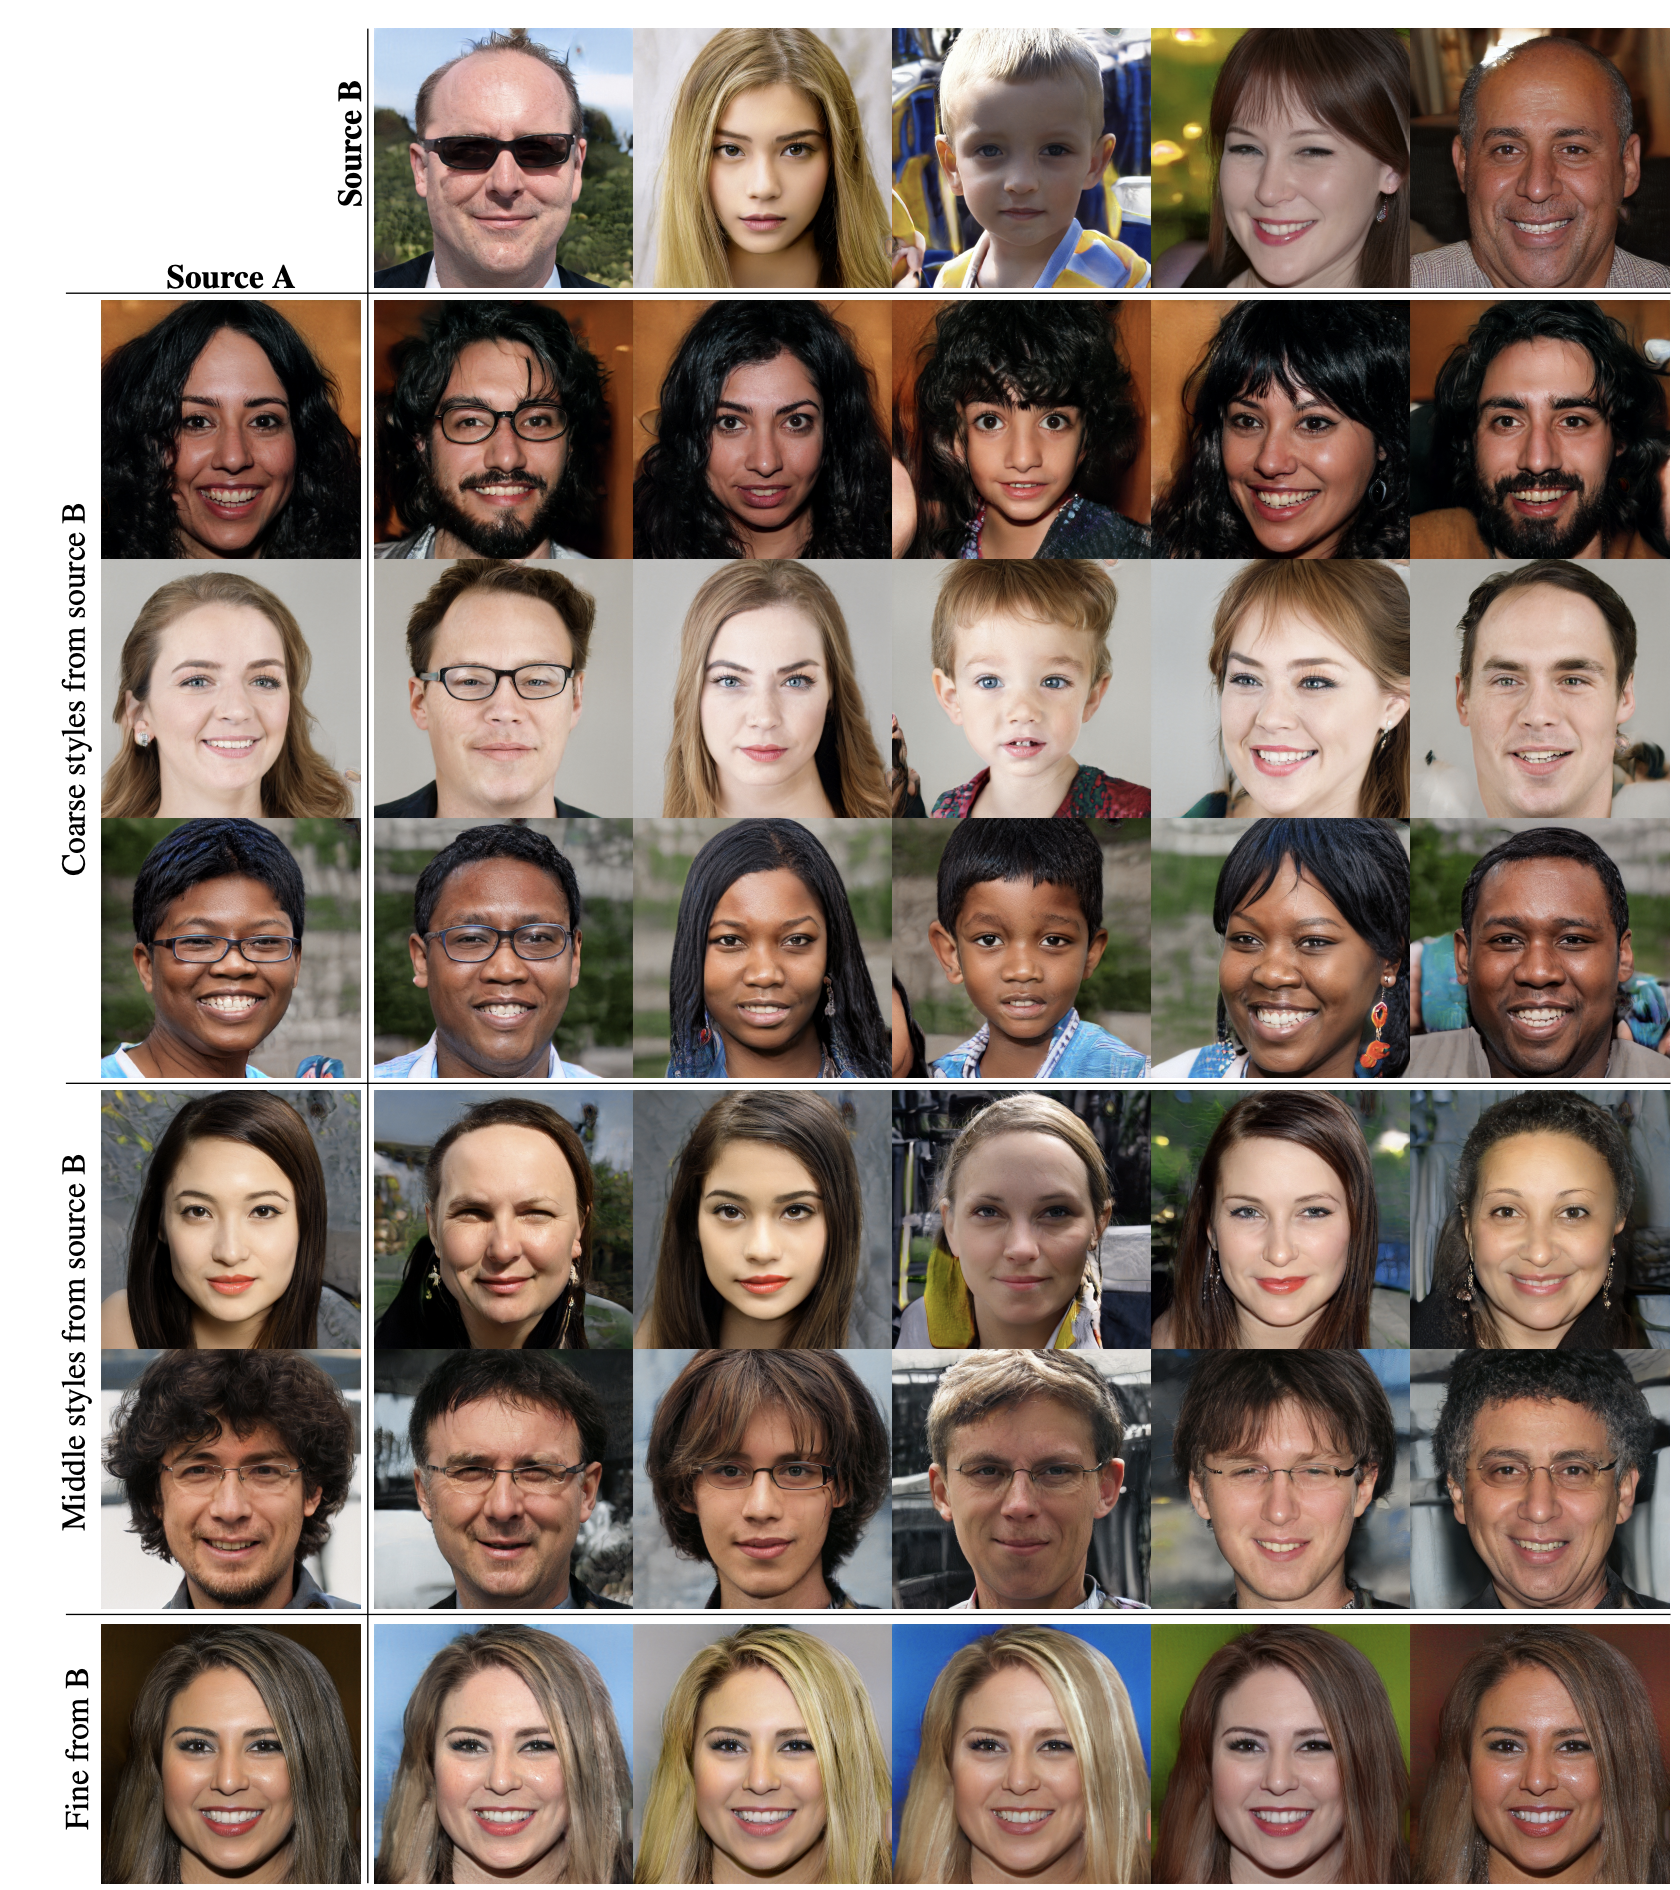
\includegraphics[height= 5.2in]{\images/Style2}}

\slide{StyleGans: Noise Variation}

\centerline{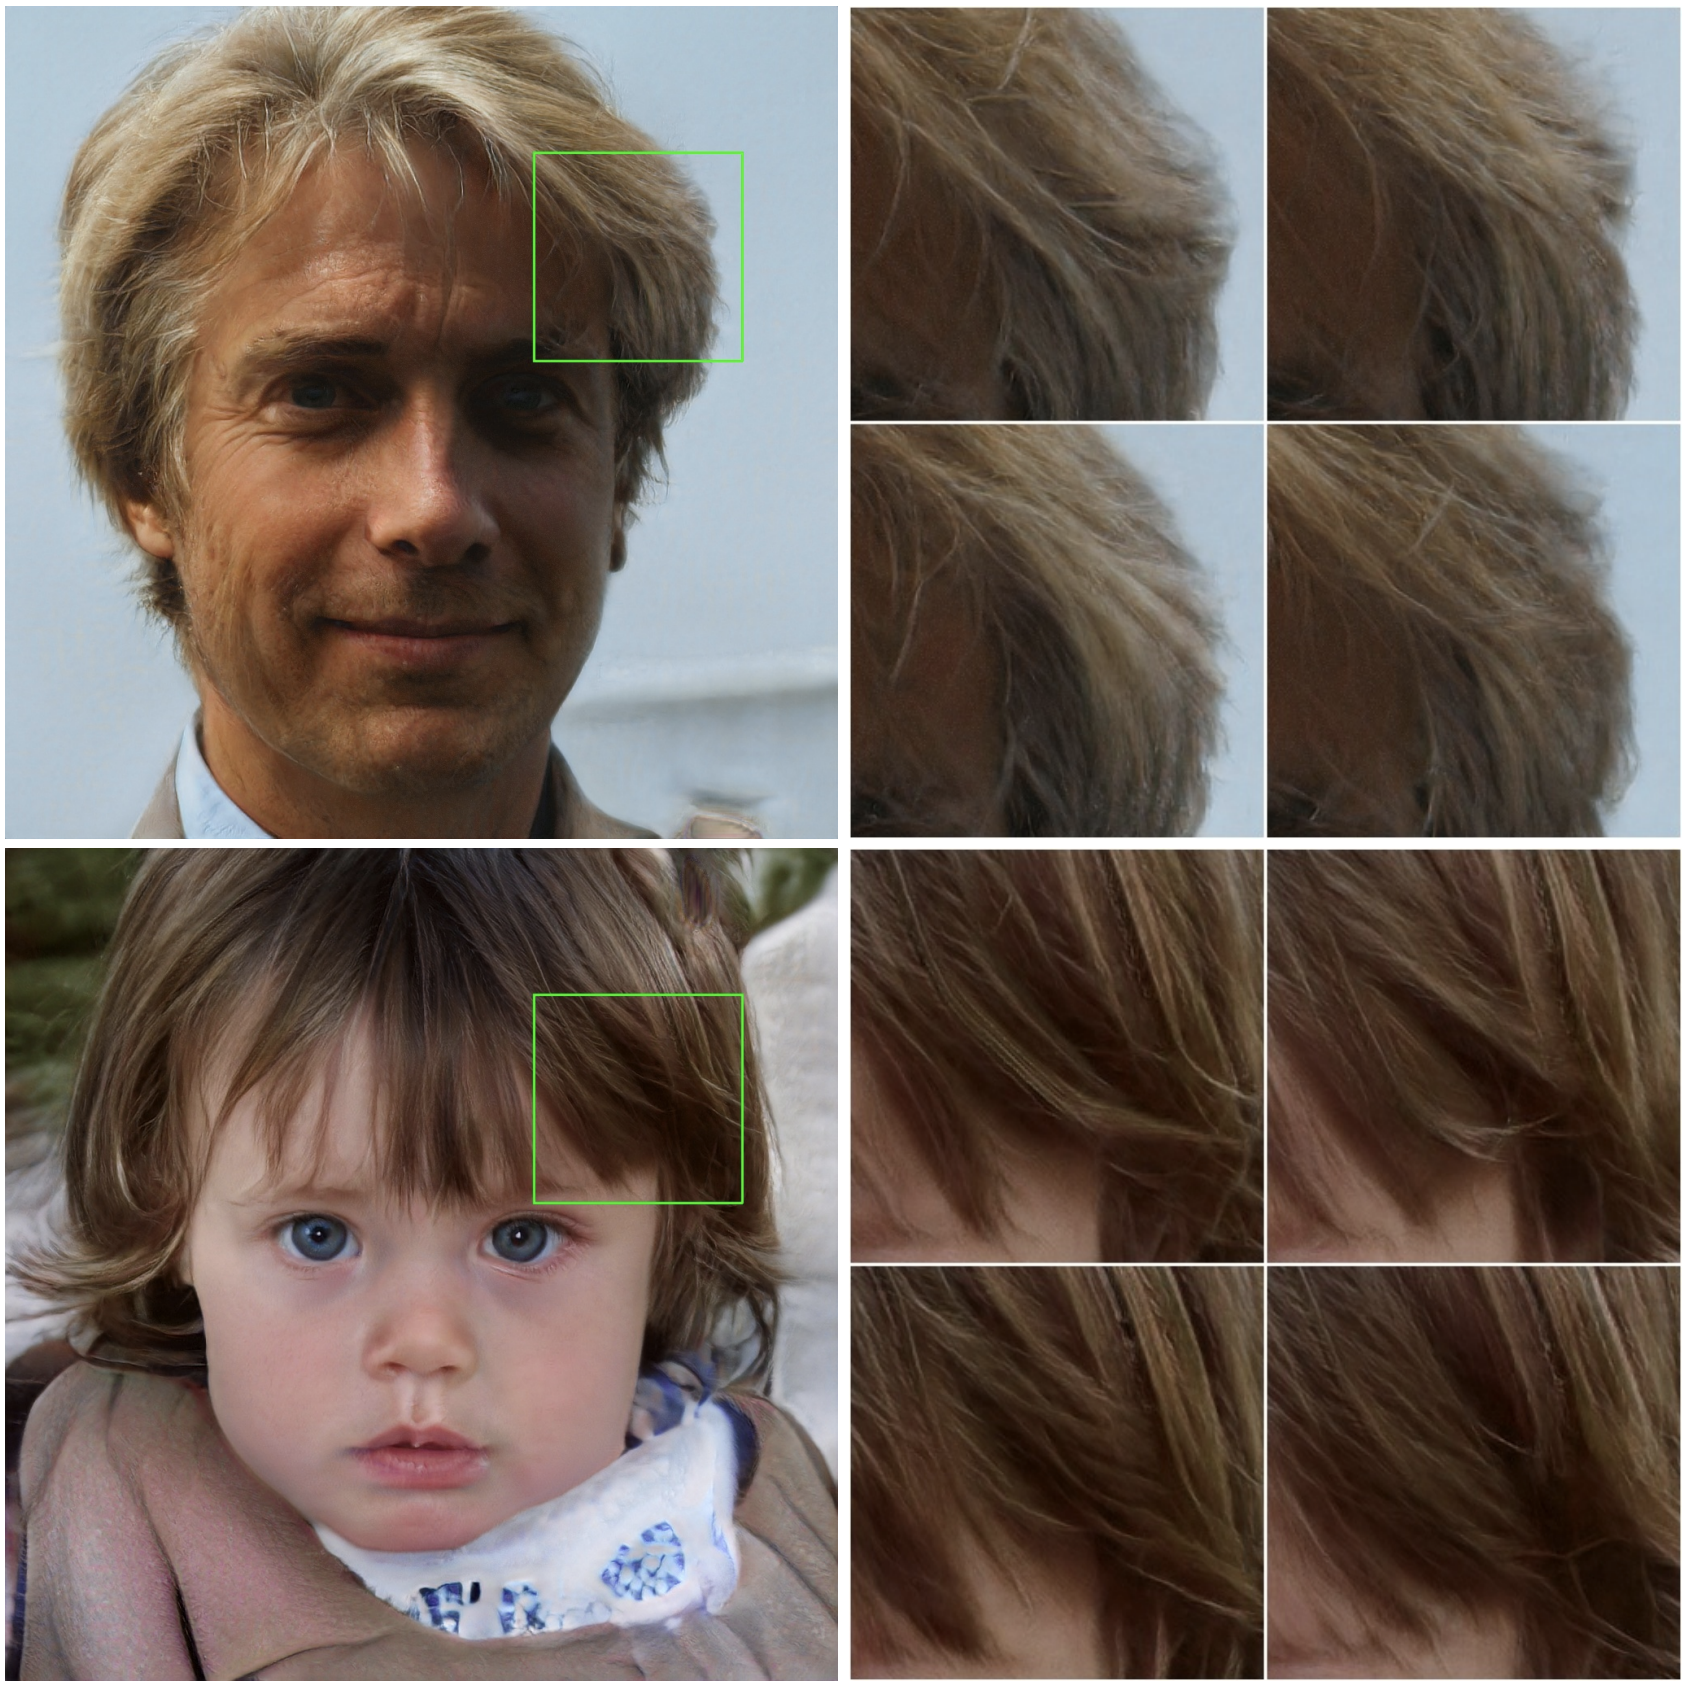
\includegraphics[height= 5.2in]{\images/Style3}}

\slide{GAN Mode Collapse}

A major concern is ``mode collapse'' where the learned distribution omits a significant fraction of the population distribution.

\vfill
There is no quantitative performance measure that provides a meaningful guarantee against mode collapse.

\slide{The Fr\'{e}nchet Inception Score (FID)}

The main problem with GANs is the lack of a meaningful quantitative evaluation metric.

\vfill
A standard quantitative performance measure is French\'{e}t Inception Distance (FID).

\vfill
This measures statistics of the features
of the inception image classification model (trained on imagenet) for images generated by the generator.

\vfill
It then compares those statistics
to the same statistics for images drawn from the population.

\vfill
But the FID score provides no guarantees against mode collapse.

\slide{GANs for Pretraining}

A main motivation for distribution modeling is to provide pre-trainined models tht can be used in downstream tasks.

\vfill
This has proved very effective in natural language processing.

\vfill
To date GANs have not proved useful for pretraining downstream applications.

\slide{END}

}
\end{document}
